下の図で簡単にCSRF攻撃の思想をご説明します

\begin{figure}[H]
   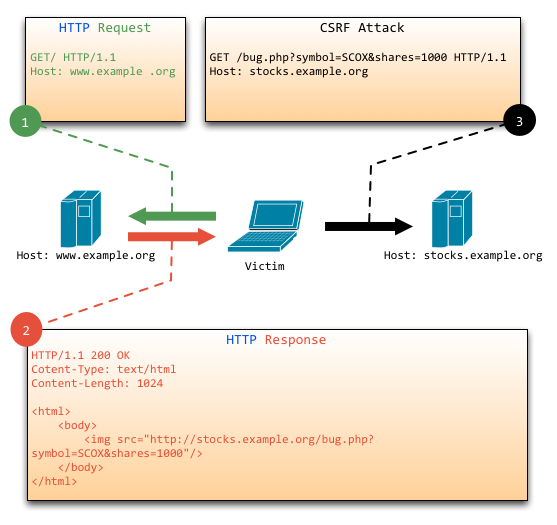
\includegraphics[width=14cm]{9.1.csrf.png}
   \label{図9.1}
   \caption{CSRFの攻撃プロセス}
\end{figure}


上の図から、CSRF攻撃を一回成功させるには被害者が2つのステップを踏まなければならないことがわかります:

\begin{enumerate}
  \item ログインがページAでの信任を受け、ローカルでCookieを生成する。
  \item Aをログアウトしていない状態で、危険なページBにアクセスする。
\end{enumerate}

ここまでで読者は次のように思われるかもしれません:"もし上の2つの条件のうち任意の一つを満足していなければ、CSRFの攻撃をうけることはない"。そうです。たしかにその通り、しかし以下の状況が発生しないことを保障することはできません:

\begin{itemize}
  \item あるページにログインしたあと、もうひとつtab画面を開き別のページにアクセスしないとは保証できません。特に最近のブラウザはどれもtabをサポートしています。
  \item ブラウザを閉じたあと、ローカルのCookieがすぐに有効期限を迎えるとは限りません。前のセッションがすでに終了していることを保証できません。
  \item 上の図で示した攻撃ページは、その他のセキュリティホールを抱えた信用できるよくアクセスされるページであることがあります。
\end{itemize}

その為、ユーザにとってあるページにログインした後なんらかのリンクをクリックしてその他の操作を避けることはとても難しいのです。ですから、いつでもCSRFの被害者になる可能性があります。

CSRF攻撃の主な原因はWebの隠された身分検証メカニズムにあります。Webの身分検証メカニズムはあるリクエストがあるユーザのブラウザからやってきたものであることを保証することはできますが、このリクエストがユーザの承認によって送信されたものであることを保証できません。
